\documentclass[a4paper,11pt]{article}
\usepackage[utf8]{inputenc}
\usepackage[T1]{fontenc}
\usepackage[french]{babel}
\usepackage[a4paper,margin=2.5cm]{geometry}
\usepackage{amsmath,amssymb}
\usepackage{graphicx}
\usepackage{float}
\usepackage{hyperref}
\usepackage{booktabs}
\usepackage{xcolor}
\usepackage{algorithm}
\usepackage[noEnd=false, indLines=true]{algpseudocodex}
\usepackage[most]{tcolorbox}

\definecolor{algobg}{RGB}{245,245,245}
\definecolor{algocomment}{RGB}{80,130,80}
\definecolor{algokeyword}{RGB}{0,50,120}
\definecolor{algoline}{RGB}{180,180,180}

\algrenewcommand\algorithmiccomment[1]{\hfill \textcolor{algocomment}{$\triangleright$ \textit{#1}}}
\algrenewcommand\algorithmicrequire{\textbf{\textcolor{algokeyword}{Entrée:}}}
\algrenewcommand\algorithmicensure{\textbf{\textcolor{algokeyword}{Sortie:}}}
\algrenewcommand\textproc{}

\newtcolorbox{algo-box}[2][]{%
	enhanced,
	width=\linewidth,
	colback=white,
	colframe=algokeyword,
	boxrule=0.5pt,
	arc=3pt,
	title={\textbf{#2}},
	coltitle=white,
	attach boxed title to top left={yshift=-2mm, xshift=2mm},
	boxed title style={colback=algokeyword, sharp corners=south},
	#1
}

\graphicspath{{images/}{graphics/}}

\title{Scout Guerlédan\\Rapport de projet}
\author{Équipe Scout}
\date{Mars 2026}

\begin{document}

\maketitle
\tableofcontents
\newpage

\section{Contexte et objectif}

\subsection{Mise en contexte}

Le projet a été mené sous la forme de séances à l'école, complétées par deux campagnes terrain au lac de Guerlédan. La première semaine sur site a été consacrée aux tests de commande des bateaux et à la mise en place d'une bibliothèque Python commune (\texttt{bblib}) afin d'uniformiser l'accès aux fonctions de communication et de pilotage. Une seconde semaine à Guerlédan a ensuite permis de focaliser le travail sur les algorithmes de localisation par intervalles et sur l'implémentation/validation de l'interface web de supervision. Le code source du projet est disponible sur le dépôt GitHub associé \cite{scout_guerledan_repo}.

Ce travail vise à localiser trois bateaux coopérant au sein d'une même flotte : un bateau-mère \texttt{MS0}, dont la position absolue (GPS) peut être connue, et deux éclaireurs \texttt{S1} et \texttt{S2} dépourvus de GPS.

Les éclaireurs peuvent ponctuellement mesurer, par acoustique, les distances inter-bateaux :
$$d_{01},\;d_{12},\;d_{20},$$
chaque mesure étant entachée d'une incertitude modélisée par des intervalles. Par ailleurs, chaque unité a connaissance, à tout instant, de l'enveloppe de la position de ses voisins sous la forme de boîtes englobantes (\textit{bounding boxes}).

Ils disposent en outre de mesures instantanées de cap et de vitesse, elles aussi incertaines. En intégrant ces mesures entre deux instants, on obtient une estimation du déplacement total avec son incertitude (dead-reckoning).

\begin{figure}[H]
\centering
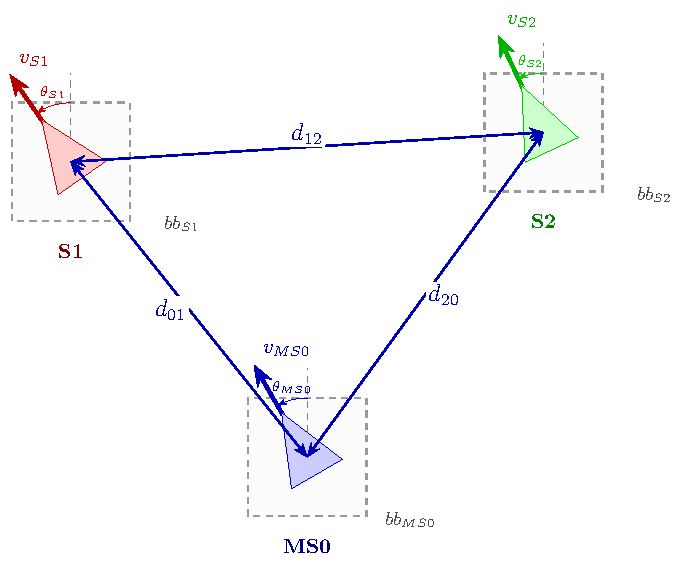
\includegraphics[width=0.78\linewidth]{schema_modelisation.pdf}
\caption{Modélisation du problème.}
\label{fig:schema_modelisation}
\end{figure}

Le cycle d'estimation est alors :
\begin{itemize}
	\item \textbf{prédiction :} propager l'ensemble des positions possibles à l'aide du déplacement dead-reckoning ;
	\item \textbf{correction :} réduire cet ensemble lorsque des mesures acoustiques et/ou GPS sont disponibles, en exploitant les distances mesurées ainsi que les boîtes englobantes des voisins.
\end{itemize}

\subsection{Objectif scientifique et technique}

L'objectif est de maintenir, pour chaque bateau, un ensemble de positions possibles cohérent avec les mesures disponibles, plutôt qu'une unique position ponctuelle qui oublierait les incertitudes. Cette approche permet de mieux gérer les erreurs de mesure et d'obtenir une estimation plus robuste. Il faudra trouver des méthodes efficaces pour réduire les incertitudes afin de les garder raisonnables.

\subsection{Matériel utilisé}

L'expérimentation repose sur :
\begin{itemize}
	\item \textbf{3 BlueBoats} (1 bateau mère + 2 éclaireurs),
	\item \textbf{1 Base Station} pour le réseau local et le pilotage,
	\item une station de calcul à terre pour l'orchestration, les logs et l'interface web.
\end{itemize}

\medskip

Nous n'avons pas réussi à avoir des modems acoustiques permettant de mesurer les distances inter-bateaux, et avons donc simulé ces mesures à l'aide des GPS des BlueBoats, en y ajoutant une incertitude pour modéliser les erreurs de mesure acoustique. Les chapitres suivants détaillent les choix de modélisation, d'algorithmes et de validation qui permettent de résoudre ce problème dans le cadre du projet.
\input{blueboat}
% ===========================================================================
% Section 3 — Bibliothèque de communication et interface de contrôle
% Auteur : Aurèle
% Packages requis dans main.tex :
%   \usepackage{booktabs, tabularx, graphicx, listings, xcolor, hyperref}
%   \usepackage[T1]{fontenc}
%   \usepackage[french]{babel}
% ===========================================================================

% Configuration des listings Python
\lstdefinestyle{python}{
  language=Python,
  basicstyle=\ttfamily\small,
  keywordstyle=\color{blue}\bfseries,
  commentstyle=\color{gray}\itshape,
  stringstyle=\color{teal},
  numberstyle=\tiny\color{gray},
  numbers=left,
  stepnumber=1,
  frame=single,
  rulecolor=\color{black!20},
  backgroundcolor=\color{black!3},
  breaklines=true,
  showstringspaces=false,
  tabsize=4,
  aboveskip=0.9em,
  belowskip=0.9em,
}

% Réglages d'espacement locaux à cette section
\newlength{\bblibOldParskip}
\newlength{\bblibOldParindent}
\newlength{\bblibOldIntextsep}
\newlength{\bblibOldTextfloatsep}
\newlength{\bblibOldAbovecaptionskip}
\newlength{\bblibOldBelowcaptionskip}
\newlength{\bblibOldAbovedisplayskip}
\newlength{\bblibOldBelowdisplayskip}
\newlength{\bblibOldAbovedisplayshortskip}
\newlength{\bblibOldBelowdisplayshortskip}

% ---------------------------------------------------------------------------
\section{Bibliothèque de communication et interface de contrôle}
\label{sec:bblib}
% ---------------------------------------------------------------------------

\setlength{\bblibOldParskip}{\parskip}
\setlength{\bblibOldParindent}{\parindent}
\setlength{\bblibOldIntextsep}{\intextsep}
\setlength{\bblibOldTextfloatsep}{\textfloatsep}
\setlength{\bblibOldAbovecaptionskip}{\abovecaptionskip}
\setlength{\bblibOldBelowcaptionskip}{\belowcaptionskip}
\setlength{\bblibOldAbovedisplayskip}{\abovedisplayskip}
\setlength{\bblibOldBelowdisplayskip}{\belowdisplayskip}
\setlength{\bblibOldAbovedisplayshortskip}{\abovedisplayshortskip}
\setlength{\bblibOldBelowdisplayshortskip}{\belowdisplayshortskip}

\setlength{\parskip}{0.55em}
\setlength{\parindent}{0pt}
\setlength{\intextsep}{13pt}
\setlength{\textfloatsep}{15pt}
\setlength{\abovecaptionskip}{9pt}
\setlength{\belowcaptionskip}{7pt}
\setlength{\abovedisplayskip}{10pt}
\setlength{\belowdisplayskip}{10pt}
\setlength{\abovedisplayshortskip}{8pt}
\setlength{\belowdisplayshortskip}{8pt}

\subsection{Contexte et motivation}
\label{sec:bblib:contexte}

\textbf{MAVLink} est le protocole de communication utilisé par ArduRover sur les BlueBoat \cite{mavlink_docs,ardurover_docs}. Il transporte des messages normalisés (par exemple \texttt{ATTITUDE}, \texttt{GLOBAL\_POSITION\_INT}, \texttt{RC\_CHANNELS\_OVERRIDE}, \texttt{COMMAND\_LONG}) identifiés par type de message et par couple (\texttt{system\_id}, \texttt{component\_id}). En usage classique, ces messages sont consommés via un flux réseau UDP/TCP maintenu en continu par le client de contrôle.

\textbf{mavlink2rest} est un serveur léger intégré à BlueOS qui fait le pont entre le flux MAVLink binaire du Pixhawk et une \textbf{API HTTP/REST} \cite{blueos_docs,mavlink2rest_docs}. Son fonctionnement est le suivant :

\begin{enumerate}
  \item Il reçoit en continu les messages MAVLink du Pixhawk via la liaison série et les stocke en mémoire (toujours le message le plus récent de chaque type).
  \item Il expose une API REST sur le port 6040 de chaque bateau, avec deux opérations :
  \begin{itemize}
    \item \texttt{GET /mavlink/vehicles/\{sysid\}/components/\{compid\}/messages/\{MSG\}} \\ retourne en JSON le dernier message reçu de ce type ;
    \item \texttt{POST /mavlink} avec un payload JSON \\ sérialise et injecte un message MAVLink dans le bus vers le Pixhawk.
  \end{itemize}
\end{enumerate}

Cette API est accessible depuis n'importe quel client HTTP sur le réseau local, sans configuration particulière. Une requête typique se présente sous cette forme :

\begin{lstlisting}[style=python, caption={Exemple de requête GET vers mavlink2rest pour lire la position GPS du bateau 2.}]
import requests
r = requests.get(
    "http://192.168.2.202:6040"
    "/mavlink/vehicles/2/components/1/messages/GLOBAL_POSITION_INT"
)
data = r.json()
lat = data["message"]["lat"] / 1e7   # conversion de 1e-7 degres vers degres
lon = data["message"]["lon"] / 1e7
\end{lstlisting}

La bibliothèque Python officielle \texttt{pymavlink} permet d'ouvrir des connexions MAVLink bas niveau (UDP, TCP, série) et d'envoyer/recevoir des messages binaires \cite{pymavlink_docs}. C'est l'approche classique. Cependant, dans notre contexte, elle présente plusieurs inconvénients majeurs.

\begin{table}[h]
  \centering
  \caption{Comparaison de \texttt{pymavlink} et \texttt{mavlink2rest} dans le contexte du projet.}
  \label{tab:mavlink_vs_rest}
  \renewcommand{\arraystretch}{1.3}
  \begin{tabular}{p{0.18\textwidth} p{0.37\textwidth} p{0.37\textwidth}}
    \toprule
    \textbf{Critère} & \textbf{\texttt{pymavlink} (socket brut)} & \textbf{\texttt{mavlink2rest} (HTTP/JSON)} \\
    \midrule
    Couche réseau
      & Socket UDP/TCP à maintenir, gestion manuelle de la reconnexion
      & Simple requête HTTP sans état \\
    Accès simultané
      & Un seul consommateur du flux (le socket draine les messages)
      & Plusieurs clients lisent le cache indépendamment \\
    Intégration BlueOS
      & BlueOS n'expose pas de socket UDP MAVLink par défaut ; configuration réseau nécessaire
      & Nativement disponible sur le port 6040, sans configuration \\
    Débogage
      & Messages binaires, outils spécialisés requis (Wireshark, logs pymavlink)
      & Testable directement avec \texttt{curl} ou un navigateur \\
    Dépendances
      & Bibliothèque lourde avec bindings C
      & Seulement \texttt{requests} (bibliothèque standard Python) \\
    Multi-bateaux
      & N sockets distincts, N threads de réception permanents
      & N instances légères d'\texttt{MavlinkLink}, sans thread réseau dédié \\
    \bottomrule
  \end{tabular}
\end{table}

Deux points sont particulièrement déterminants dans notre cas. D'abord, l'aspect \textbf{multi-clients} : pendant les tests, l'interface de supervision, les scripts de mission et les modules de logging tournent en parallèle sur la station de base, chacun devant accéder aux données des trois bateaux. Avec un socket MAVLink, le flux est consommé par le premier lecteur ; avec mavlink2rest, chaque composant interroge indépendamment le cache. Ensuite, l'aspect \textbf{intégration BlueOS} : sans modifier la configuration de BlueOS, aucun socket UDP MAVLink n'est publié vers l'extérieur, tandis que l'API REST est disponible sans intervention.

Les différents scripts du projet — tests unitaires, scripts de mission, interface graphique, boucle de localisation — partagent tous les mêmes opérations fondamentales : lire le GPS, envoyer une commande moteur, lire le cap. Sans abstraction commune, chaque script réimplémenterait les requêtes HTTP, le parsing JSON MAVLink et les conversions de coordonnées, multipliant les sources d'erreurs et les duplications de code.

La bibliothèque \textbf{\texttt{bblib}} (\textit{BlueBoat Library}) centralise cette logique sous une API orientée objet cohérente. Elle est testable indépendamment des bateaux physiques grâce au simulateur \texttt{fake\_mavlink2rest.py} décrit à la section~\ref{sec:bblib:fake}.

% ---------------------------------------------------------------------------
\subsection{Architecture de \texttt{bblib.py}}
\label{sec:bblib:arch}
% ---------------------------------------------------------------------------

\texttt{bblib.py} est organisé en cinq classes principales, dont les dépendances sont résumées ci-dessous :

\begin{center}
\ttfamily
\begin{tabular}{l}
MavlinkLink \\
\quad $\hookrightarrow$ IMU \\
\quad $\hookrightarrow$ GPS $\longrightarrow$ geo\_conversion \\
\quad $\hookrightarrow$ MotorDriver \\
\quad $\hookrightarrow$ Navigation(IMU, GPS, MotorDriver) \\[4pt]
BlueBoatConfig $\longrightarrow$ init\_blueboat() $\longrightarrow$ (MavlinkLink, IMU, GPS, MotorDriver, Navigation)
\end{tabular}
\end{center}

\noindent Les paramètres globaux (gain proportionnel $K_p$, période d'échantillonnage $\Delta t$, commande maximale) sont centralisés dans \texttt{utils/settings.py} pour éviter les constantes dispersées dans le code.

\label{sec:bblib:mavlinklink}
\texttt{MavlinkLink} est la seule classe à interagir directement avec le réseau. Elle encapsule une session \texttt{requests.Session} et fournit une interface haut niveau au reste de la bibliothèque.

Ses paramètres de construction sont l'adresse IP du bateau (\texttt{host}), le port mavlink2rest (\texttt{port}, par défaut 6040), les identifiants MAVLink (\texttt{sysid}, \texttt{compid}) et un délai d'attente (\texttt{timeout}). L'option \texttt{silent\_errors} permet de supprimer les messages d'erreur dans les threads de monitoring qui tolèrent les coupures réseau passagères.

Les méthodes principales sont :

\begin{itemize}
  \item \texttt{get\_message(msg\_name)} : requête \texttt{GET} vers l'endpoint mavlink2rest ; retourne le dictionnaire JSON du dernier message de ce type, ou \texttt{None} en cas d'échec.
  \item \texttt{post\_message(message)} : requête \texttt{POST} avec le payload encapsulé dans un header MAVLink (\texttt{system\_id} = 255, identifiant habituel d'une station sol GCS).
  \item \texttt{send\_rc\_override(ch1, ch3)} : construit et envoie un message \texttt{RC\_CHANNELS\_OVERRIDE} pour les canaux 1 (throttle) et 3 (steering).
  \item \texttt{arm\_disarm(arm)} : envoi de \texttt{MAV\_CMD\_COMPONENT\_ARM\_DISARM}.
  \item \texttt{set\_flight\_mode(mode\_id/mode\_name)} : changement de mode ArduRover (\texttt{MANUAL}, \texttt{GUIDED}, \texttt{AUTO}…) via une table de correspondance nom $\leftrightarrow$ identifiant numérique.
  \item \texttt{get\_flight\_mode()} : lecture du mode actuel et de l'état armé/désarmé depuis le message \texttt{HEARTBEAT}.
  \item \texttt{get\_battery\_status()} : lecture de la tension, du courant et du pourcentage restant depuis \texttt{BATTERY\_STATUS} et \texttt{SYS\_STATUS}.
\end{itemize}

La classe \texttt{IMU} lit l'orientation du bateau depuis le message MAVLink \texttt{ATTITUDE}, qui transmet les angles de roulis, tangage et lacet calculés par le filtre EKF (\textit{Extended Kalman Filter}) embarqué dans ArduRover.

\texttt{get\_euler\_angles()} retourne le triplet $(\phi, \theta, \psi)$ en radians. Un cache interne (\texttt{\_last\_euler}) conserve la dernière valeur valide, de sorte que la méthode ne retourne jamais \texttt{None} après la première lecture réussie, même lors de micro-coupures réseau.

\texttt{get\_attitude\_dict()} retourne un dictionnaire enrichi incluant \texttt{yaw\_deg}, le cap normalisé dans $[0^\circ, 360^\circ]$, directement exploitable par la couche Navigation.

La classe \texttt{GPS} lit la position du bateau depuis deux sources MAVLink possibles, par ordre de priorité :
\begin{enumerate}
  \item \texttt{GLOBAL\_POSITION\_INT} : position fusionnée par l'EKF (latitude, longitude, altitude, cap) ; valeurs entières en $10^{-7}$ degrés, à diviser par $10^7$.
  \item \texttt{GPS\_RAW\_INT} : données brutes du récepteur GNSS, utilisé en fallback si le premier message n'est pas disponible.
\end{enumerate}

\texttt{get\_gps()} retourne la position sous forme de tuple \texttt{(lat, lon)} en degrés décimaux et maintient un historique horodaté dans \texttt{gps\_history}.

\texttt{get\_coords()} retourne les coordonnées \textbf{cartésiennes locales} $(x, y)$ en mètres, via la fonction \texttt{geo\_conversion.conversion\_spherique\_cartesien()} qui effectue une projection sphérique autour d'un point de référence \texttt{POINT\_BASE} défini dans \texttt{settings.py} (ici, le quai de Guerlédan). Cette représentation est celle utilisée par l'algorithme de localisation par intervalles.

\texttt{export\_gpx(filename)} exporte la trace GPS au format GPX horodaté, compatible avec les logiciels SIG (QGIS, Google Maps) pour la visualisation des trajectoires.

Le BlueBoat est propulsé par deux moteurs (gauche et droit) contrôlés par des signaux PWM (\textit{Pulse-Width Modulation}) entre 1000 et 2000~µs, le neutre étant à 1500~µs. \texttt{MotorDriver} traduit des commandes de haut niveau en surcharges de canaux RC.

La conversion d'une paire de commandes moteur $(left, right) \in [-C_{max}, C_{max}]$ en signaux PWM se fait via la décomposition throttle/steering :
\[
  t = \frac{L + R}{2}, \qquad s = \frac{R - L}{2}
\]
\[
  \text{CH1} = 1500 - 500\,t, \qquad \text{CH3} = 1500 + 500\,s
\]

Les méthodes principales sont \texttt{send\_cmd\_motor(left, right)} pour un envoi instantané, \texttt{drive\_lr(left, right, seconds, rate\_hz)} pour une commande maintenue pendant une durée donnée (avec retour automatique au neutre), et \texttt{stop\_motors()} pour interrompre immédiatement la propulsion. Pour la sécurité, le destructeur \texttt{\_\_del\_\_} coupe les moteurs et désarme le véhicule.

\label{sec:bblib:navigation}
La classe \texttt{Navigation} réalise la boucle de guidage du bateau. Elle repose sur un \textbf{régulateur proportionnel} sur l'erreur de cap :
\[
  e = \psi_{\text{cible}} - \psi_{\text{actuel}} \quad (\text{normalisée dans } {[-180^\circ, 180^\circ]})
\]
\[
  \text{correction} = K_p \cdot e, \qquad \begin{cases} \text{moteur gauche} = v_{\text{base}} - \text{correction} \\ \text{moteur droit} = v_{\text{base}} + \text{correction} \end{cases}
\]

Plusieurs modes de navigation sont disponibles :

\begin{itemize}
  \item \texttt{follow\_heading(target\_heading\_deg, duration\_s)} : suivi d'un cap fixe pendant une durée donnée, à vitesse constante.
  \item \texttt{go\_to\_gps(target\_coords, distance)} : navigation vers un waypoint GPS avec une loi de vitesse de rapprochement $v = v_{\text{base}} \cdot \tanh(d / d_{\text{ref}})$, permettant un ralentissement progressif à l'approche.
  \item \texttt{go\_to\_position(target)} : commande vectorielle instantanée (1-shot) vers une position cartésienne locale. Cette méthode est utilisée pour l'intégration avec la boucle de l'algorithme de localisation.
  \item \texttt{return\_home()} : séquence de waypoints prédéfinis vers la zone d'amarrage de Guerlédan.
  \item \texttt{stay\_at(point)} : maintien de position par rappel doux.
\end{itemize}

Pour éviter de coder les adresses IP en dur dans les scripts, la configuration de la flotte est externalisée dans un fichier JSON (\texttt{boat\_control\_config.json}) :

\begin{lstlisting}[style=python, caption={Exemple de fichier de configuration de la flotte (\texttt{boat\_control\_config.json}).}]
[
  {"boat_id": 1, "host": "192.168.2.201", "port": 6040, "sysid": 1},
  {"boat_id": 2, "host": "192.168.2.202", "port": 6040, "sysid": 2},
  {"boat_id": 3, "host": "192.168.2.203", "port": 6040, "sysid": 3}
]
\end{lstlisting}

La classe \texttt{BlueBoatConfig} charge ce fichier avec des valeurs par défaut en cas d'absence. La méthode \texttt{init\_from\_config}, appelée avec l'argument \texttt{boat\_id}, instancie en une seule ligne l'ensemble des composants d'un bateau (\texttt{MavlinkLink}, \texttt{IMU}, \texttt{GPS}, \texttt{MotorDriver}, \texttt{Navigation}). \texttt{init\_all()} parcourt tous les bateaux configurés et retourne un dictionnaire indexé par \texttt{boat\_id}, utilisé par les scripts de mission multi-bateaux.

% ---------------------------------------------------------------------------
\subsection{Interface graphique de supervision — \texttt{boat\_control\_gui.py}}
\label{sec:bblib:gui}
% ---------------------------------------------------------------------------

Pour les essais terrain, l'équipe avait besoin d'un outil permettant de surveiller l'état des bateaux en temps réel et d'envoyer des commandes simples sans passer par la ligne de commande. L'interface \texttt{boat\_control\_gui.py} répond à ce besoin. Elle est entièrement construite sur \texttt{bblib}, ce qui valide en pratique que la bibliothèque couvre l'ensemble des cas d'usage (figure~\ref{fig:boat_control_gui}).

\begin{figure}[h]
  \centering
  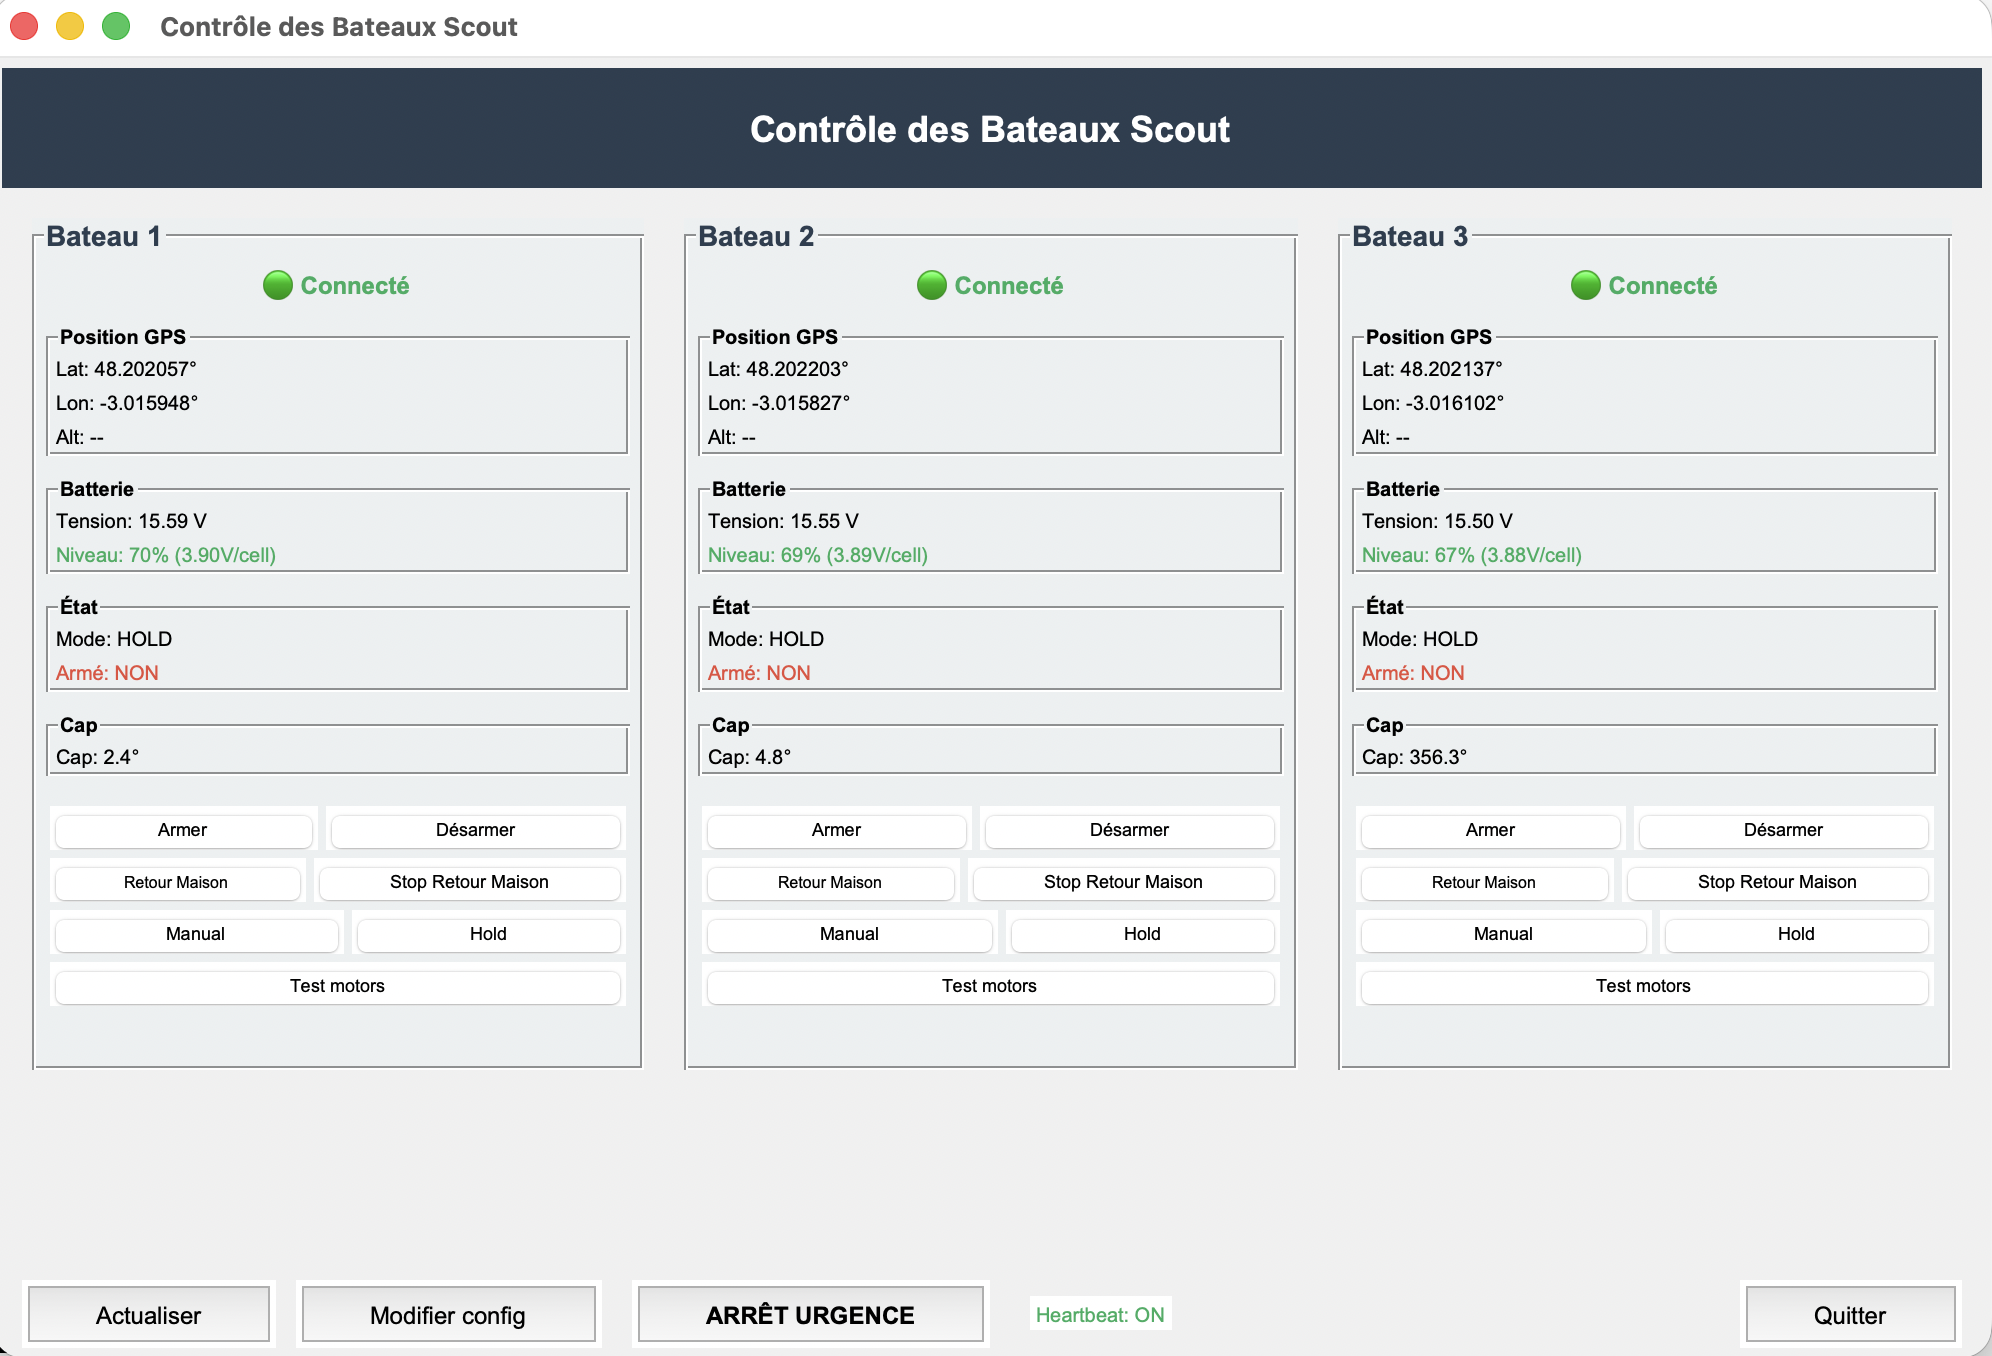
\includegraphics[width=0.85\textwidth]{images/boat_control_python.png}
  \caption{Interface graphique de supervision et de contrôle des trois bateaux (\texttt{boat\_control\_gui.py}).}
  \label{fig:boat_control_gui}
\end{figure}

Le protocole MAVLink exige qu'une station sol (GCS) envoie régulièrement un message \texttt{HEARTBEAT} pour signaler sa présence. Si BlueOS ne reçoit pas de heartbeat depuis la station pendant plusieurs secondes, il peut désarmer le véhicule ou couper la connexion. Le \texttt{HeartbeatManager} lance un thread dédié qui envoie ce message à 1~Hz vers chacun des bateaux configurés, en parallèle de toute autre activité de l'interface.

Un objet \texttt{BoatMonitor} est instancié pour chaque bateau. Il encapsule les composants \texttt{bblib} du bateau correspondant et lance un thread de polling à environ 2~Hz qui met à jour en continu les données affichées : position GPS, cap, tension et pourcentage de batterie, mode ArduRover et état armé/désarmé. La détection du nombre de cellules de la batterie (3S ou 4S) est automatique à partir de la tension mesurée, ce qui permet de calculer un pourcentage fiable sans configuration manuelle.

L'interface est organisée en panneaux, un par bateau, affichant :
\begin{itemize}
  \item \textbf{GPS} : latitude et longitude en degrés décimaux ;
  \item \textbf{Cap} : heading en degrés, mis à jour depuis l'\texttt{IMU} ;
  \item \textbf{Batterie} : tension en volts et pourcentage estimé ;
  \item \textbf{Mode} : mode ArduRover actif et indicateur armé/désarmé.
\end{itemize}

Des boutons permettent d'\textbf{armer}, de \textbf{désarmer} et de lancer un \textbf{retour maison} (exécuté dans un thread séparé via \texttt{Navigation.return\_home()} pour ne pas bloquer l'interface). La configuration est chargée dynamiquement depuis \texttt{boat\_control\_config.json} : il suffit de modifier les adresses IP dans ce fichier pour adapter l'interface à un autre réseau. Enfin, les connexions indisponibles sont gérées explicitement : un bateau hors réseau affiche des valeurs dégradées sans bloquer les autres panneaux.

% ---------------------------------------------------------------------------
\subsection{Simulateur \texttt{fake\_mavlink2rest.py}}
\label{sec:bblib:fake}
% ---------------------------------------------------------------------------

Pour permettre le développement et les tests sans accès physique aux bateaux, un serveur HTTP simulant l'API mavlink2rest a été développé dans \texttt{fake\_mavlink2rest.py}. Il démarre un serveur HTTP léger par port (un par bateau simulé), chacun générant des données synthétiques :
\begin{itemize}
  \item Position GPS animée autour d'un point de base avec bruit gaussien ;
  \item Attitude (roll, pitch, yaw) avec bruit et dérive ;
  \item Tension de batterie décroissante au fil du temps ;
  \item Gestion des commandes \texttt{POST} : armement, changement de mode, RC override.
\end{itemize}

Ce simulateur a été particulièrement utilisé pendant la deuxième semaine pour valider plus rapidement l'interface et exécuter des tests de type SITL de manière simple. Par rapport à un SITL ArduRover complet, il est plus léger à mettre en œuvre : au lieu de simuler toute la pile ArduRover et l'ensemble MAVLink, il se contente de renvoyer des réponses HTTP/JSON cohérentes avec les endpoints attendus par nos scripts. Ce compromis accélère fortement les tests d'intégration de \texttt{bblib} et de l'interface sans mobiliser le matériel.

% ---------------------------------------------------------------------------
\subsection{Tests de la première semaine}
\label{sec:bblib:tests}
% ---------------------------------------------------------------------------

Le script \texttt{test\_bblib.py} fournit une interface en ligne de commande pour tester chaque fonctionnalité de \texttt{bblib} de manière isolée, en se connectant soit au simulateur soit à un bateau réel. Le tableau~\ref{tab:test_bblib} résume les commandes disponibles.

\begin{table}[h]
  \centering
  \caption{Commandes du script de test \texttt{test\_bblib.py}.}
  \label{tab:test_bblib}
  \renewcommand{\arraystretch}{1.3}
  \begin{tabular}{p{0.24\textwidth} p{0.70\textwidth}}
    \toprule
    \textbf{Commande} & \textbf{Fonctionnalité testée} \\
    \midrule
    \texttt{imu}         & Lecture du message \texttt{ATTITUDE} → roll / pitch / yaw en radians et degrés \\
    \texttt{gps}         & Lecture de \texttt{GLOBAL\_POSITION\_INT} ou \texttt{GPS\_RAW\_INT} → lat/lon/alt/cap \\
    \texttt{arm}         & Armement du véhicule via \texttt{MAV\_CMD\_COMPONENT\_ARM\_DISARM} \\
    \texttt{disarm}      & Désarmement du véhicule \\
    \texttt{battery}     & Lecture de la tension et du pourcentage de batterie \\
    \texttt{neutral}     & Envoi d'un RC override neutre (CH1=CH3=1500~µs) \\
    \texttt{drive}       & Commande moteurs pendant $N$ secondes à gauche/droite spécifiés \\
    \texttt{heading}     & Suivi de cap avec le régulateur proportionnel \\
    \texttt{goto}        & Navigation vers un waypoint GPS \\
    \texttt{config}      & Chargement et affichage de \texttt{boat\_control\_config.json} \\
    \bottomrule
  \end{tabular}
\end{table}

Plusieurs scripts complémentaires ont été développés durant cette première semaine :

\begin{itemize}
  \item \textbf{\texttt{test\_mavlinkrest.py}} : tests bas niveau de l'interface REST — vérification des codes HTTP, structure des réponses JSON, latences de requêtes GET et POST.
  \item \textbf{\texttt{test\_set\_mode\_manual.py}} : validation de la commande de changement de mode ArduRover.
  \item \textbf{\texttt{test\_load\_config.py}} : vérification du parsing JSON et des valeurs par défaut de \texttt{BlueBoatConfig}.
  \item \textbf{\texttt{test\_multiple\_boat.py}} : initialisation simultanée des trois bateaux et polling en parallèle pour valider l'absence de blocage.
  \item \textbf{\texttt{test\_formation\_triangle.py}} : premier essai de formation en triangle (voir figure~\ref{fig:test_formation}), utilisant \texttt{go\_to\_position()} sur les trois bateaux coordonnés depuis la station de base.
\end{itemize}

\begin{figure}[h]
  \centering
  \includegraphics[width=0.6\textwidth]{images/test_formation.png}
  \caption{Photo de deux BlueBoat dans l'eau lors d'un essai de déplacement en formation.}
  \label{fig:test_formation}
\end{figure}

Les tests ont permis de valider le bon fonctionnement de l'ensemble de la chaîne de communication. Quelques points de vigilance ont été identifiés :

\begin{itemize}
  \item \textbf{Latence REST} : chaque requête \texttt{GET} vers mavlink2rest prend typiquement 50 à 100~ms sur le réseau WiFi local. Cela impose une fréquence de contrôle maximale d'environ 10~Hz pour la boucle de guidage, ce qui s'est avéré suffisant pour la dynamique lente des bateaux.
  \item \textbf{Heartbeat obligatoire} : sans l'envoi régulier du \texttt{HEARTBEAT} GCS, BlueOS refusait les commandes RC override. Le \texttt{HeartbeatManager} a été développé en réponse directe à ce comportement observé lors des premiers tests.
  \item \textbf{Robustesse réseau} : les coupures WiFi passagères sont gérées par l'option \texttt{silent\_errors} de \texttt{MavlinkLink} et le cache interne de l'\texttt{IMU}, qui évitent les exceptions non contrôlées dans les threads de monitoring.
  \item \textbf{Précision GPS} : la précision observée est de l'ordre de 1 à 3~mètres, cohérente avec du GPS standard sans correction différentielle.
\end{itemize}

Cette première phase s'est conclue par la validation d'un déplacement en formation de deux BlueBoat, utilisé comme test d'intégration final de \texttt{bblib} avant les essais terrain.

% ---------------------------------------------------------------------------
\subsection{Bilan}
\label{sec:bblib:bilan}
% ---------------------------------------------------------------------------

La bibliothèque \texttt{bblib} fournit une abstraction complète de la communication MAVLink/REST pour les BlueBoat. Son API orientée objet a permis de développer rapidement et de façon fiable l'interface de supervision, les scripts de mission multi-bateaux et la boucle d'intégration avec l'algorithme de localisation par intervalles décrit à la section~\ref{sec:interval}.

Le choix de mavlink2rest plutôt que pymavlink s'est avéré particulièrement judicieux dans ce contexte : il supprime toute gestion de socket, permet un accès multi-clients naturel et exploite l'API déjà exposée par BlueOS. La contrepartie — une latence légèrement plus élevée qu'un accès UDP direct — reste négligeable au regard de la dynamique des bateaux de surface.

\setlength{\parskip}{\bblibOldParskip}
\setlength{\parindent}{\bblibOldParindent}
\setlength{\intextsep}{\bblibOldIntextsep}
\setlength{\textfloatsep}{\bblibOldTextfloatsep}
\setlength{\abovecaptionskip}{\bblibOldAbovecaptionskip}
\setlength{\belowcaptionskip}{\bblibOldBelowcaptionskip}
\setlength{\abovedisplayskip}{\bblibOldAbovedisplayskip}
\setlength{\belowdisplayskip}{\bblibOldBelowdisplayskip}
\setlength{\abovedisplayshortskip}{\bblibOldAbovedisplayshortskip}
\setlength{\belowdisplayshortskip}{\bblibOldBelowdisplayshortskip}

\input{interval}
\section{Tests, validation et interface web}

\subsection{Objectif de la campagne de tests}

Cette section documente la validation de l'algorithme intervalle selon un enchaînement progressif :
\begin{enumerate}
	\item validation fonctionnelle des briques de communication,
	\item observation en simulation/rejeu,
	\item validation en conditions réelles sur les BlueBoats.
\end{enumerate}

L'objectif est de vérifier à la fois la cohérence logicielle de la chaîne complète et le comportement de l'estimation en présence d'incertitudes réelles (GPS, cap, distances).

\subsection{Interface web de supervision}

Le projet intègre une interface Django (dossier \texttt{web\_interface}) avec trois vues principales :
\begin{itemize}
	\item \textbf{Manager de flotte} : configuration des bateaux, visualisation GPS, actions de contrôle ;
	\item \textbf{Observation intervalles} : exécution pas-à-pas de l'algorithme avec affichage des boîtes et pavages ;
	\item \textbf{Logs viewer} : rejeu temporel des logs et visualisation des sorties de prédiction.
\end{itemize}

Les routes API associées (\texttt{/api/boats/*}, \texttt{/api/interval/*}, \texttt{/api/replay/*}, \texttt{/api/logs/*}) permettent d'unifier pilotage, enregistrement, rejeu et analyse.

\begin{figure}[H]
	\centering
	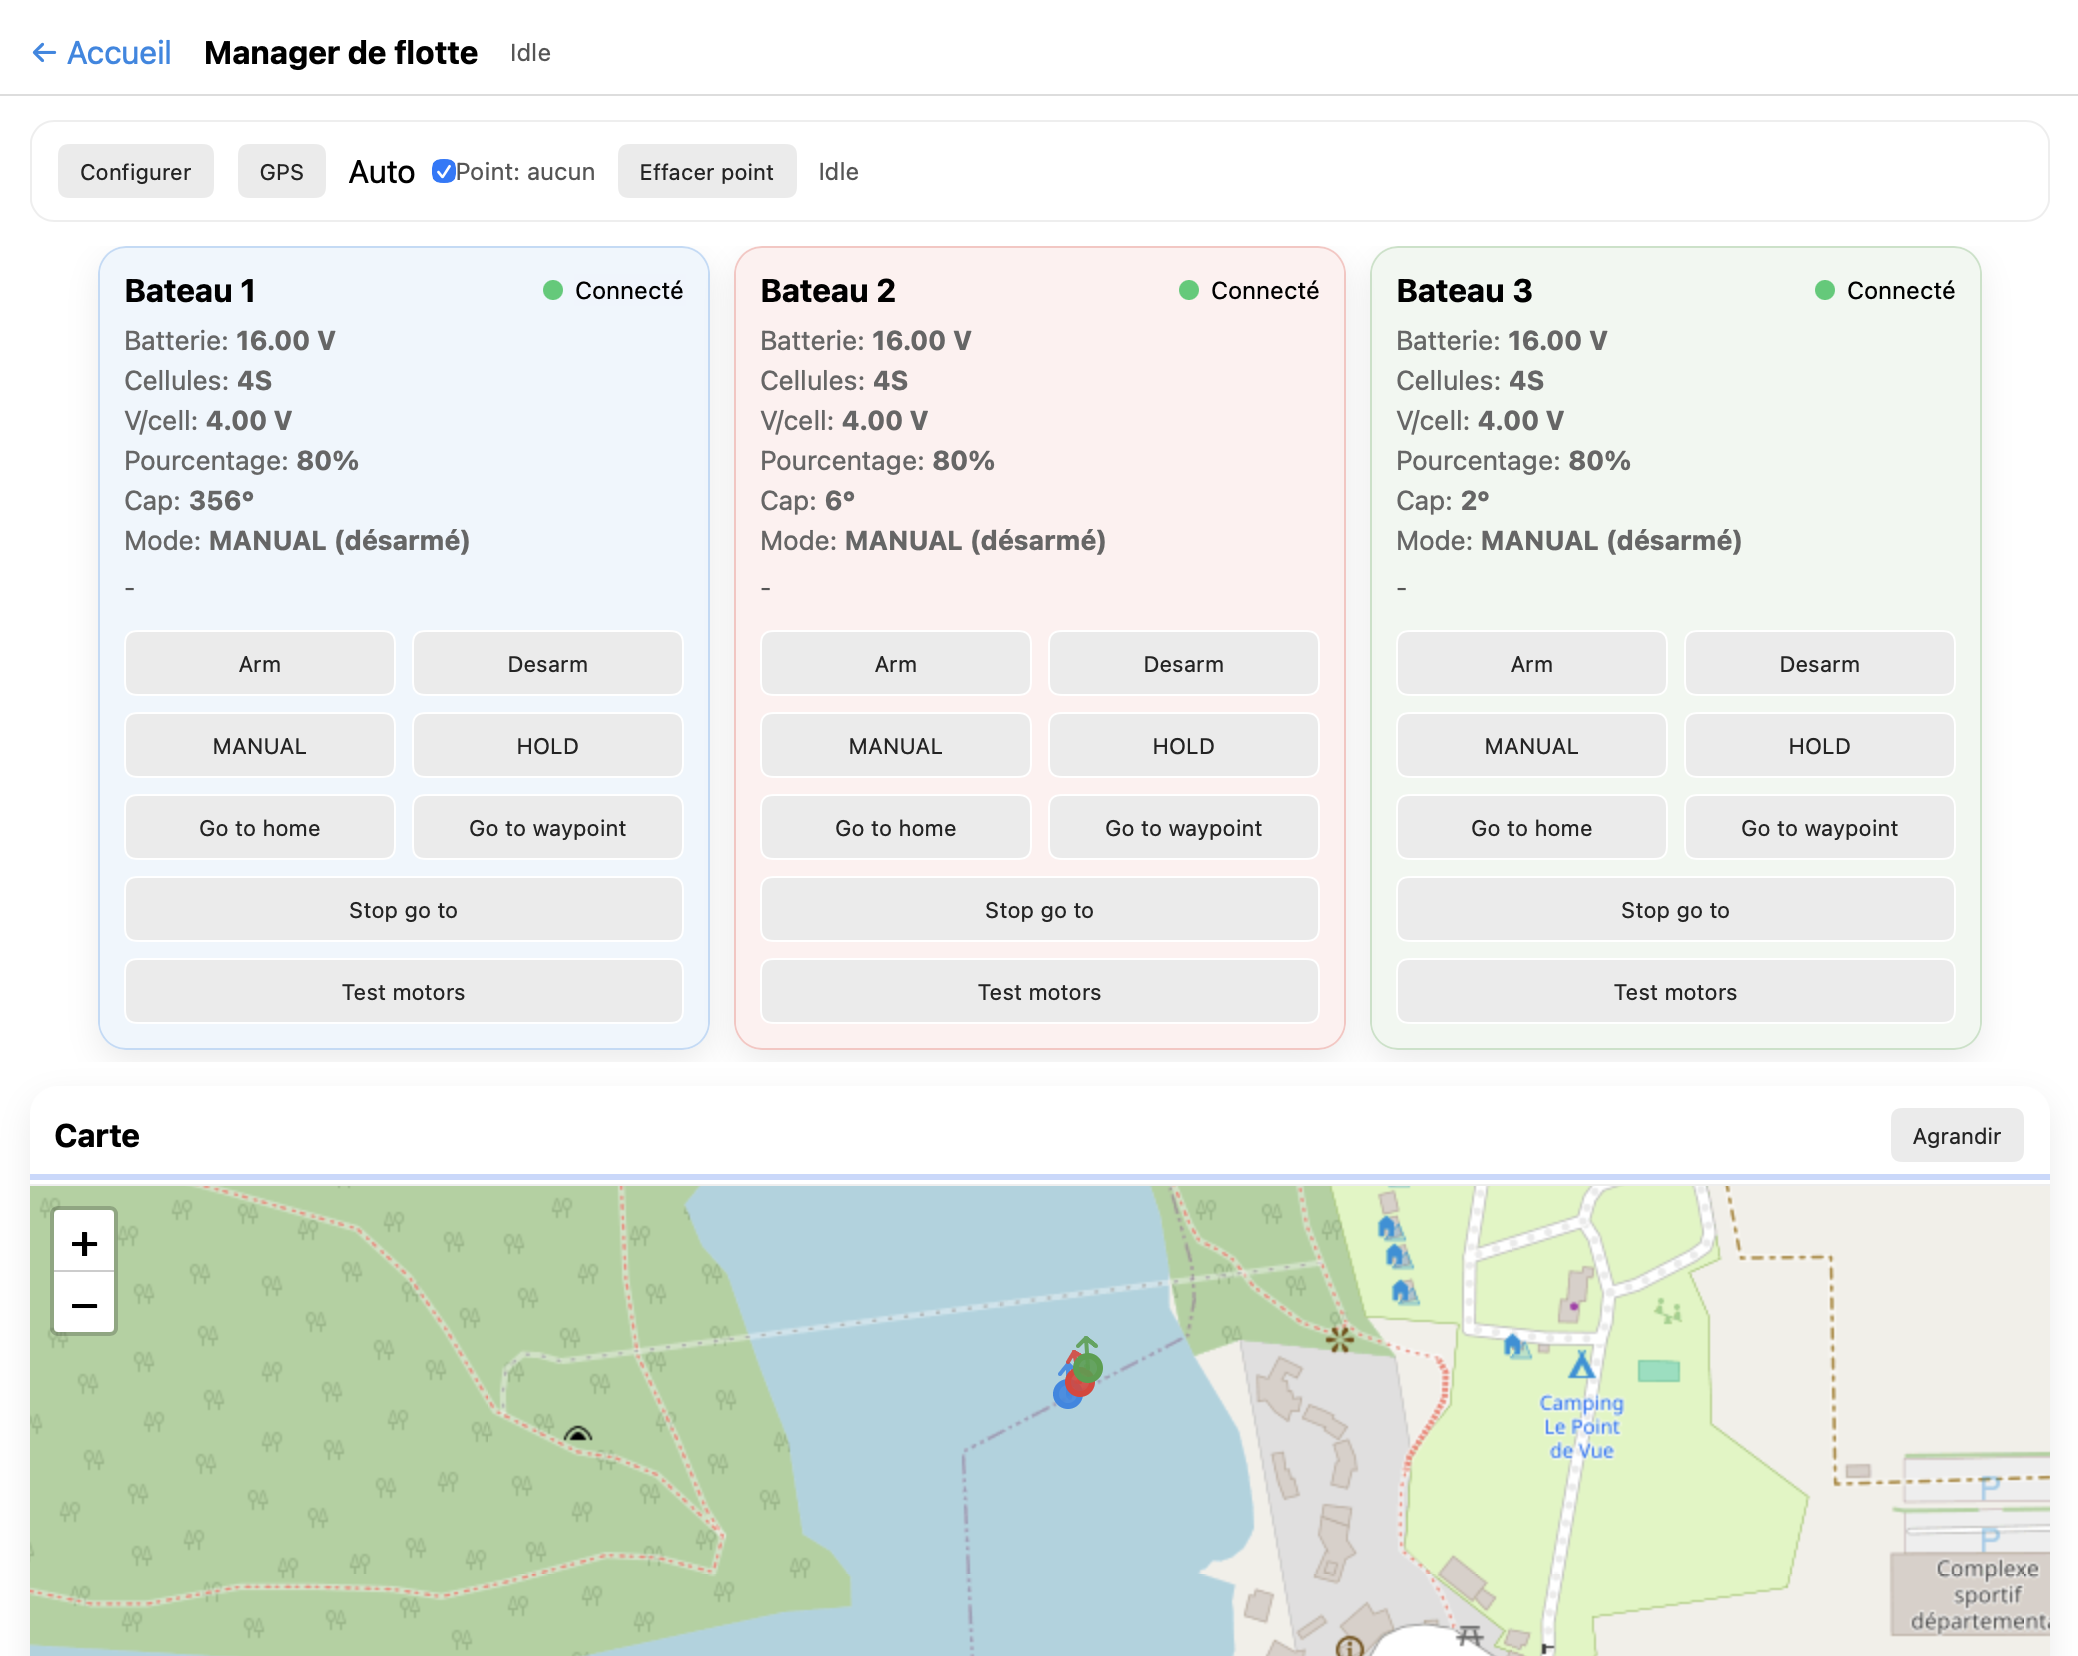
\includegraphics[width=0.82\linewidth]{interface_web/manager.png}
	\caption{Vue \textit{Manager de flotte} : configuration des bateaux, état et contrôle.}
	\label{fig:web_manager}
\end{figure}

\subsection{Observation de l'algorithme intervalle en ligne}

La page \texttt{/interval/} fournit un mode d'observation en temps réel avec paramètres réglables :
\begin{itemize}
	\item \texttt{init\_uncertainty}, \texttt{gps\_uncertainty}, \texttt{dist\_uncertainty}, \texttt{move\_uncertainty},
	\item précision de pavage et marge d'affichage,
	\item mode récursif ou non récursif.
\end{itemize}

À chaque itération, l'endpoint \texttt{/api/interval/step/} retourne :
\begin{itemize}
	\item les positions GPS des trois bateaux,
	\item les boîtes courantes des contracteurs,
	\item les polygones de pavage des deux éclaireurs.
\end{itemize}

Cette boucle de visualisation permet de diagnostiquer rapidement les réglages d'incertitude et d'observer la contraction des ensembles en fonction des mesures disponibles.

\begin{figure}[H]
	\centering
	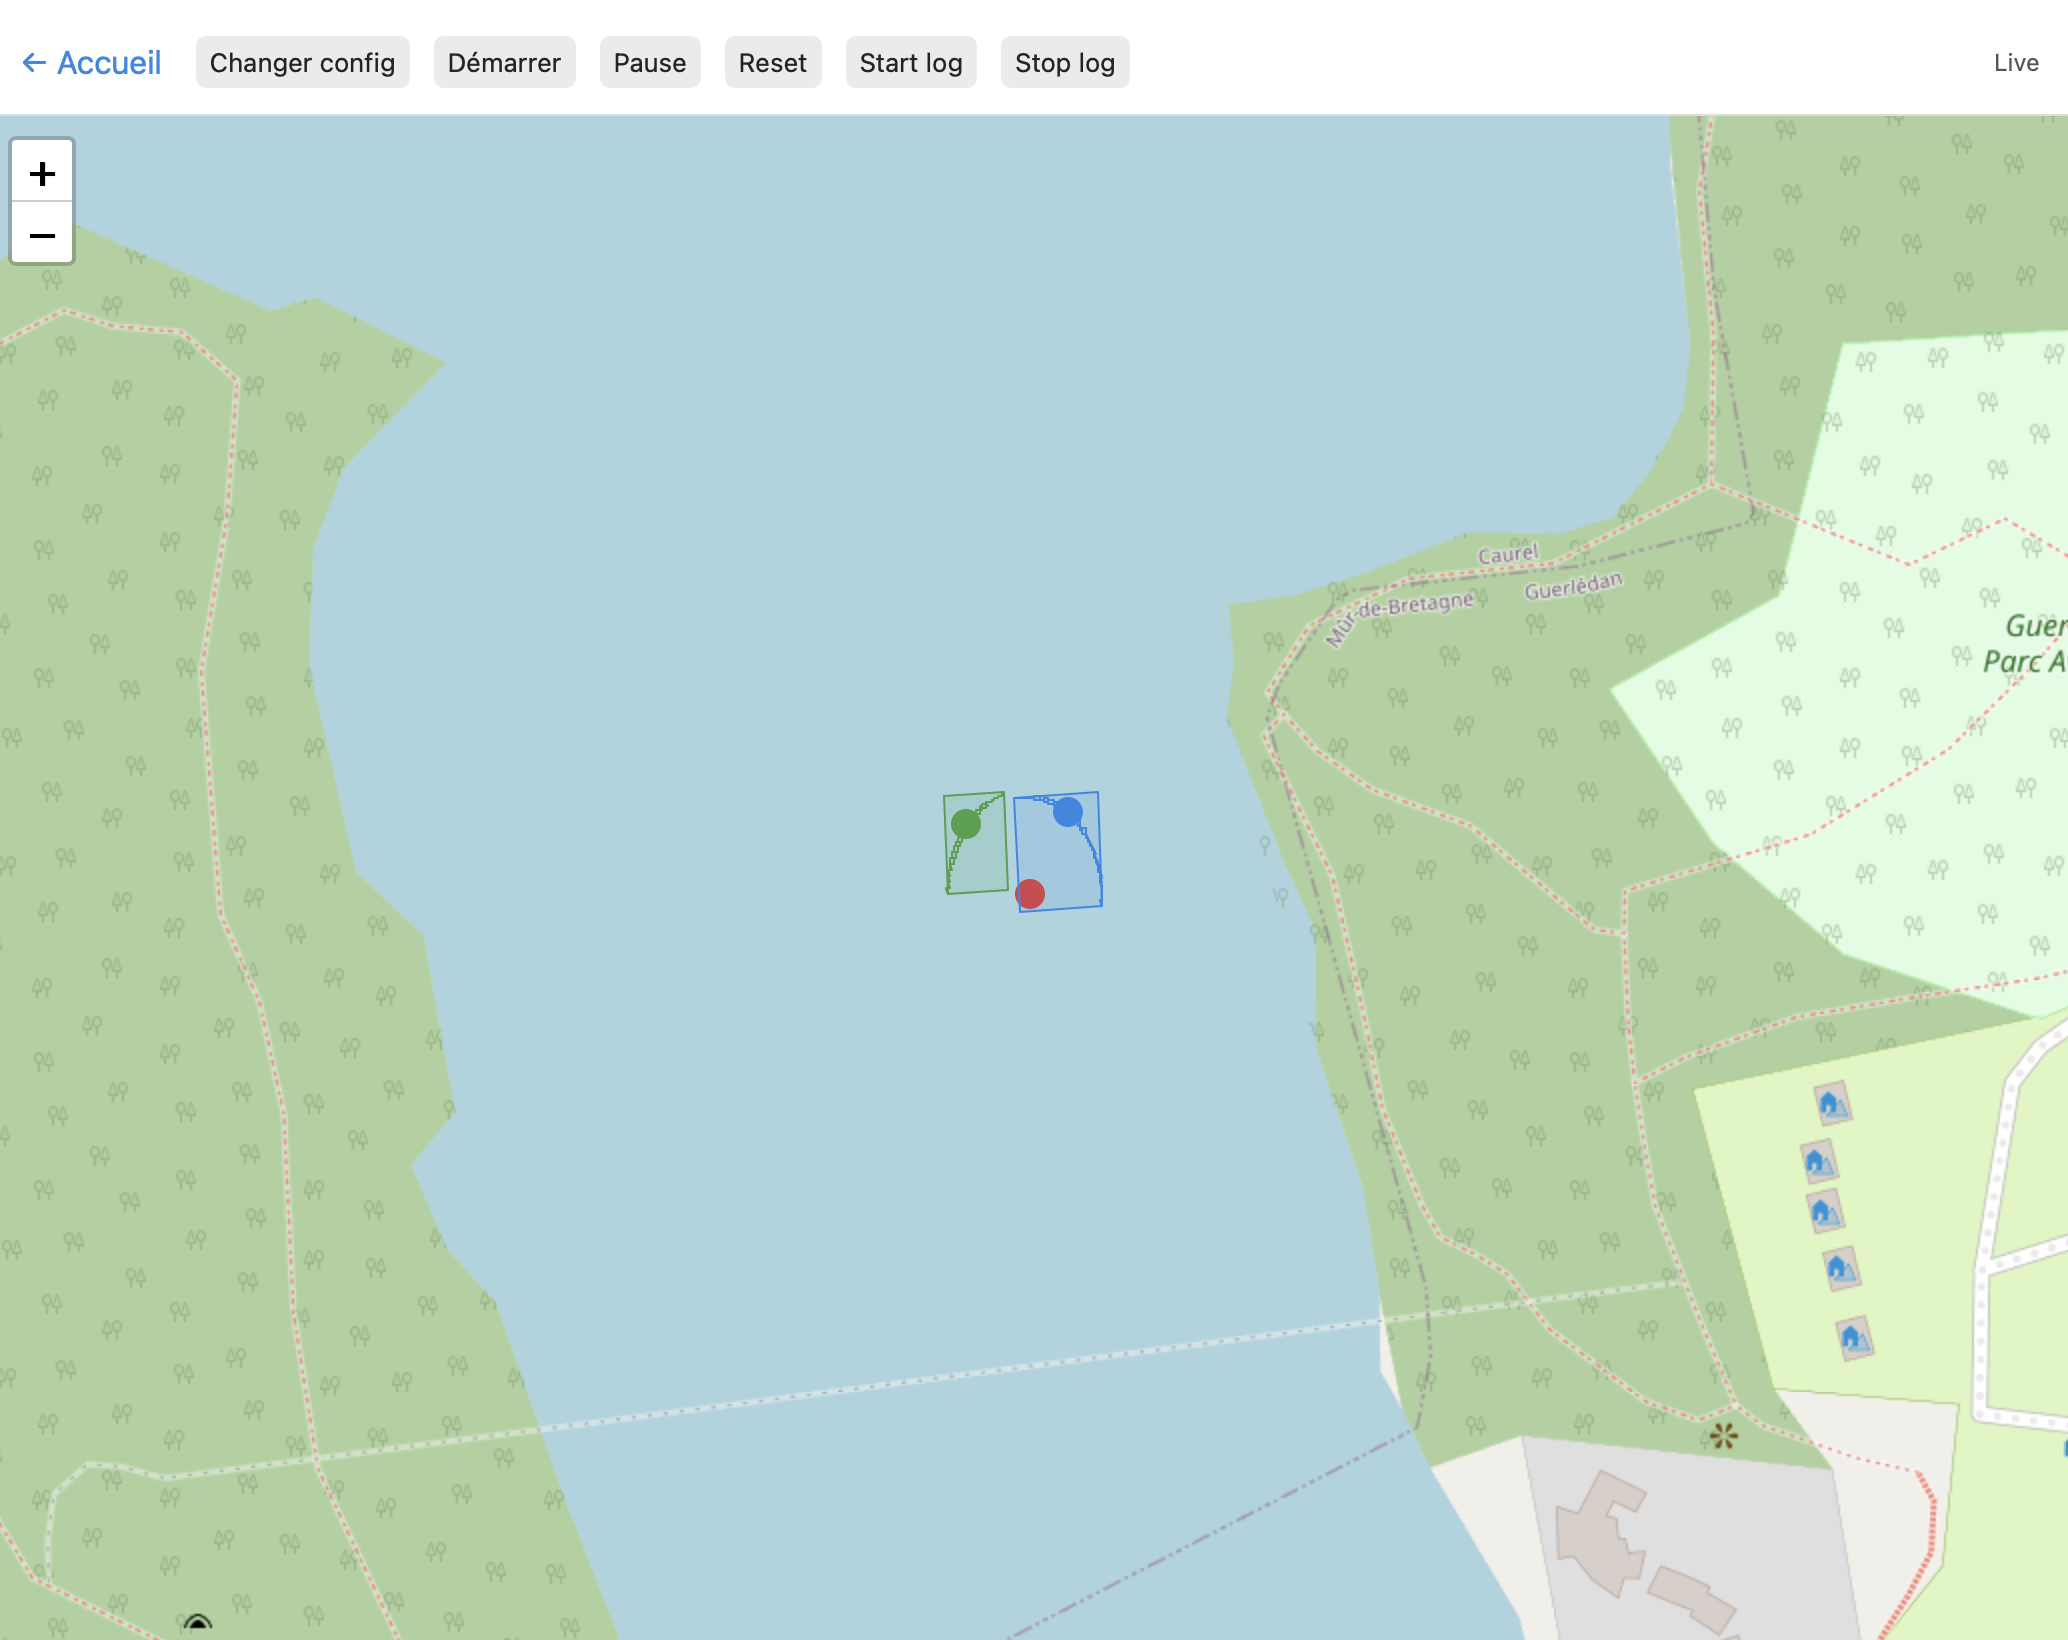
\includegraphics[width=0.82\linewidth]{interface_web/observer.png}
	\caption{Vue \textit{Observation intervalles} : boîtes et pavages en temps réel.}
	\label{fig:web_observer}
\end{figure}

\subsection{Rejeu de logs et reproductibilité}

La vue \texttt{/logs/} permet de charger un fichier de log, d'appliquer un facteur de sous-échantillonnage et de rejouer l'expérience avec un curseur temporel. Ce mode est utilisé pour :
\begin{itemize}
	\item comparer plusieurs jeux de paramètres sur une même trace,
	\item vérifier la stabilité du pipeline hors conditions terrain,
	\item produire des figures et analyses reproductibles pour le rapport.
\end{itemize}

\begin{figure}[H]
	\centering
	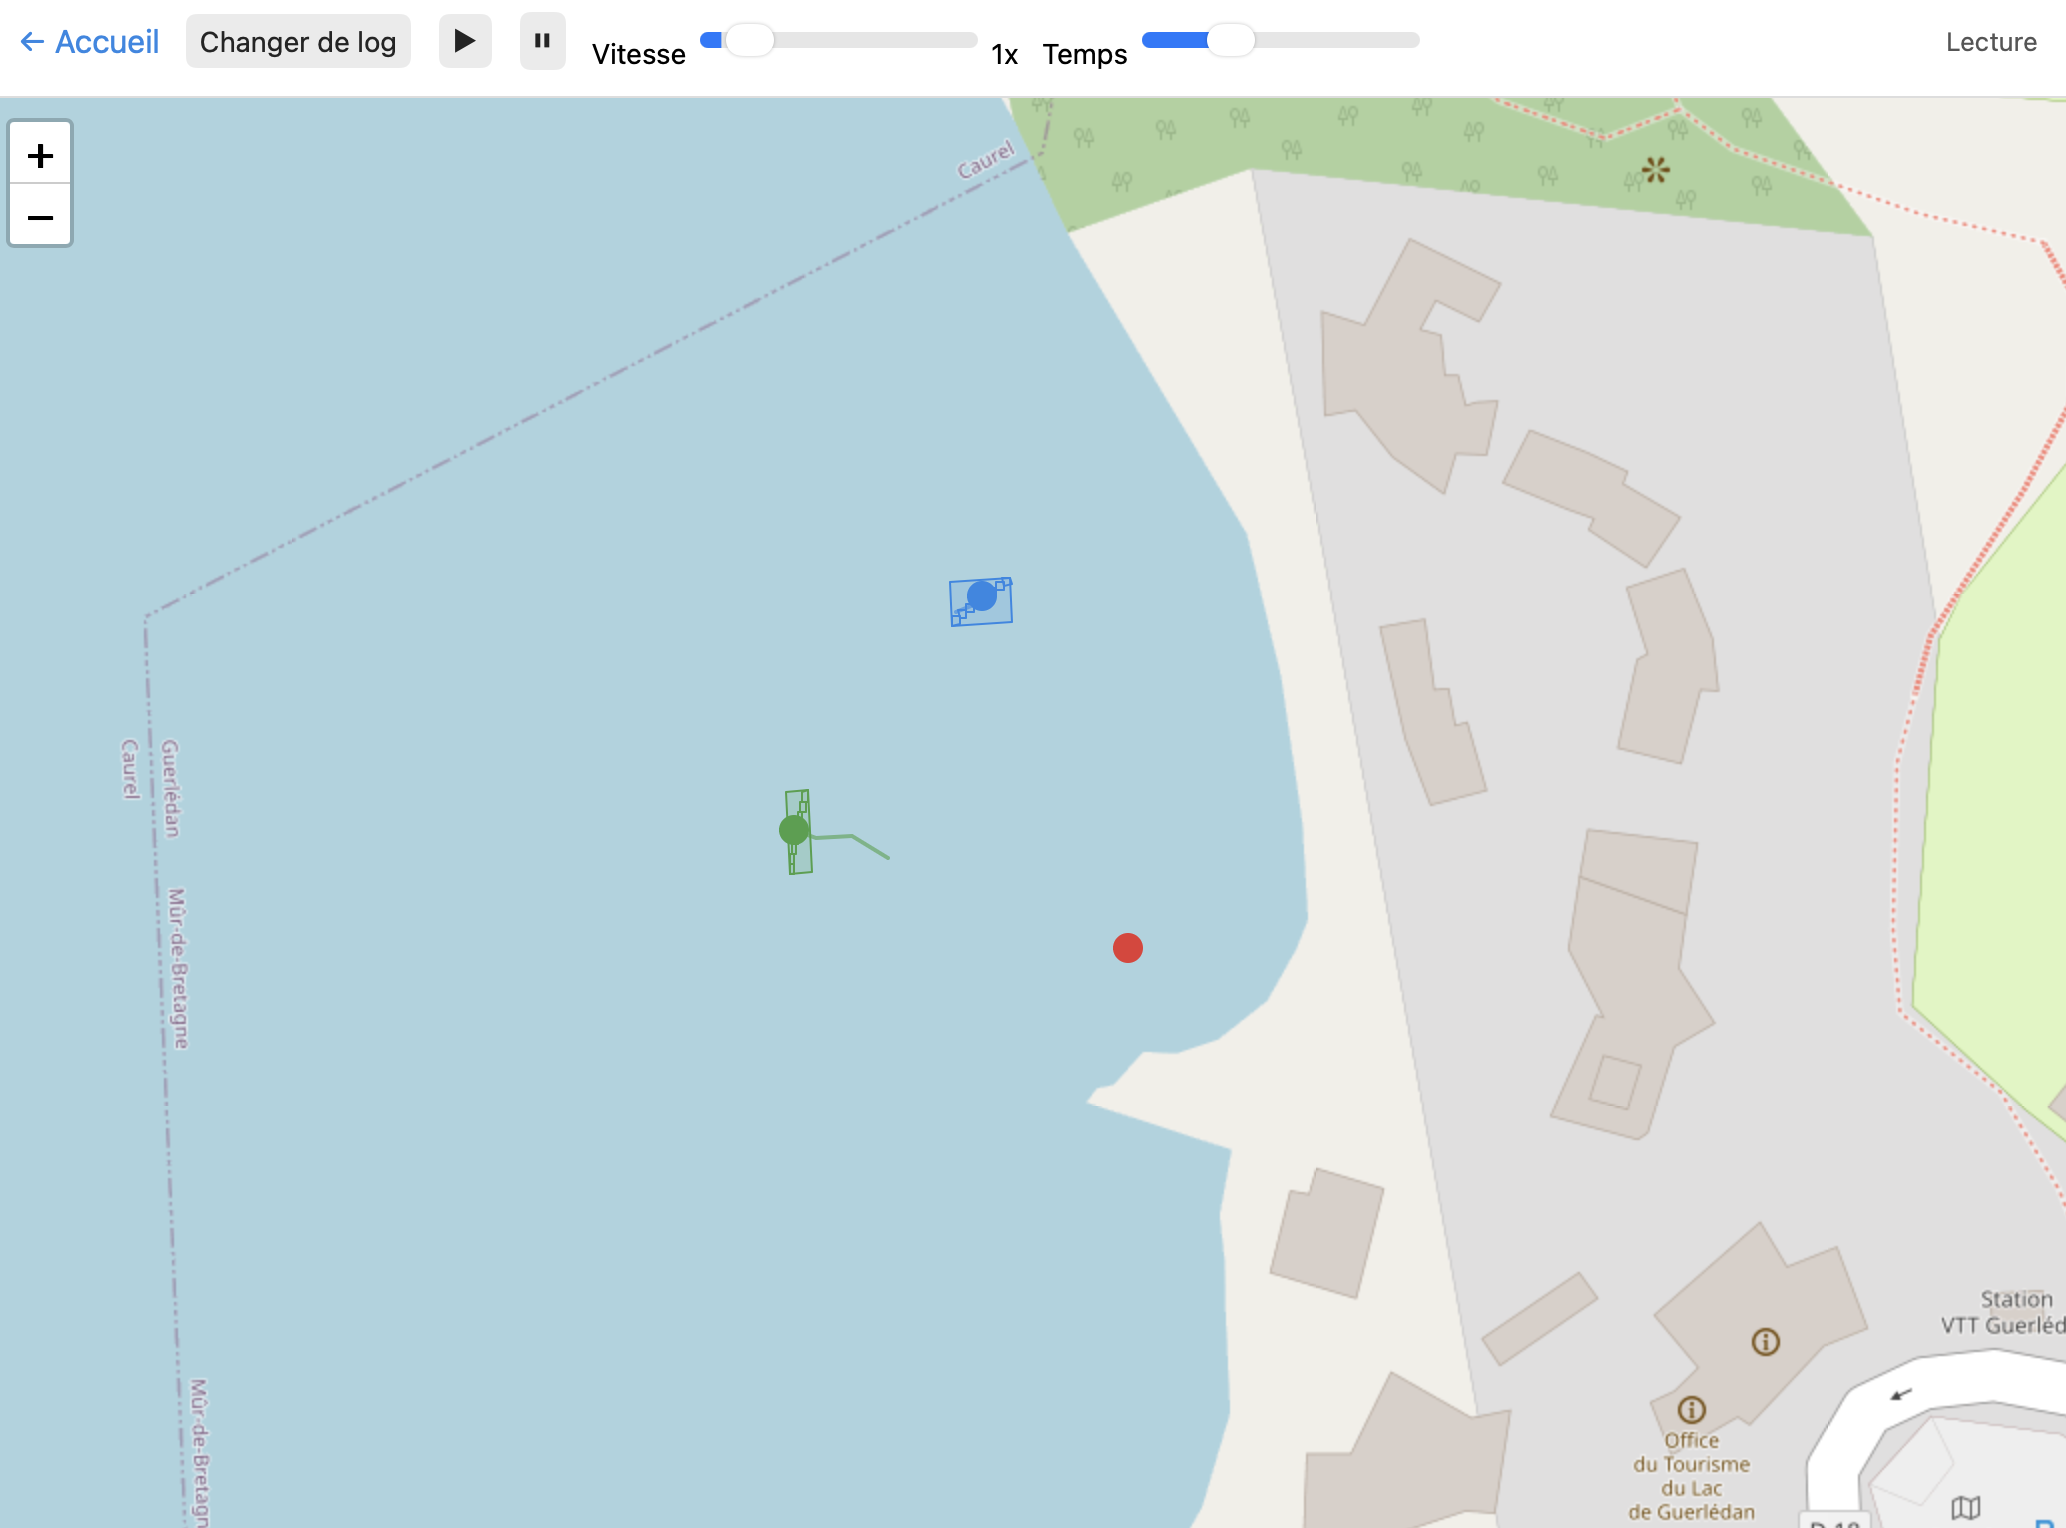
\includegraphics[width=0.82\linewidth]{interface_web/replay.png}
	\caption{Vue \textit{Replay} : rejeu temporel des logs et analyse des trajectoires.}
	\label{fig:web_replay}
\end{figure}

\subsection{Tests de comportement flotte (simulation/terrain)}

Les scripts de test du dépôt couvrent plusieurs scénarios représentatifs :
\begin{itemize}
	\item \texttt{test\_multiple\_boat.py} : exécution simultanée de deux bateaux (cap imposé + poursuite),
	\item \texttt{test\_formation\_triangle.py} : génération de cibles pour maintenir une formation triangulaire,
	\item \texttt{test\_mavlinkrest.py}, \texttt{test\_load\_config.py}, \texttt{test\_set\_mode\_manual.py} : vérification des briques de communication et de configuration.
\end{itemize}

La validation est réalisée d'abord avec des données contrôlées (rejeu/simulation), puis avec les données acquises sur les BlueBoats. Cette progression limite les risques opérationnels et facilite l'identification des causes d'erreur.

\begin{figure}[H]
	\centering
	\includegraphics[width=0.70\linewidth]{test_formation.png}
	\caption{Exemple de test de formation utilisé pour valider le comportement collectif.}
	\label{fig:test_formation}
\end{figure}

\subsection{Validation de l'évitement de singularité}

La stratégie retenue consiste à éviter les géométries dégénérées au niveau des trajectoires et à renforcer la correction par fusion multi-contraintes. En pratique, les scénarios de test ont confirmé les points suivants :
\begin{itemize}
	\item lorsque les bateaux restent trop alignés, les ensembles estimés s'étirent et la localisation devient moins discriminante ;
	\item dès qu'une excitation latérale est introduite (triangle, suivi avec variation de cap), l'intersection des contraintes se resserre ;
	\item la combinaison distances + boîte GPS du bateau mère + boîtes voisins réduit significativement l'ambiguïté.
\end{itemize}

Ces observations sont cohérentes avec l'analyse théorique de la section précédente et valident l'approche pratique retenue pour éviter les cas mal conditionnés.

\section{Résultats, limites et perspectives}

Ce projet a permis de valider une chaîne complète, depuis la communication avec les BlueBoats jusqu'à l'observation de la localisation par intervalles en simulation et en conditions réelles. Les résultats obtenus montrent que l'approche est exploitable opérationnellement : l'estimation reste cohérente, la visualisation est utilisable sur le terrain, et l'algorithme non récursif supprime la contrainte de temps de calcul qui limitait les premières versions.

Les essais confirment également un point central : la qualité de localisation dépend fortement de la géométrie de flotte. Une configuration triangulaire maintenue trop longtemps conduit à une inflation progressive des ensembles admissibles. À l'inverse, des manoeuvres d'échappement introduites au bon moment permettent de contracter les boîtes et de restaurer une incertitude plus faible.

\subsection{Bilan synthétique}

Les contributions principales du groupe sont les suivantes :
\begin{itemize}
	\item mise en place d'une bibliothèque de contrôle/navigation robuste pour les BlueBoats ;
	\item intégration d'une interface web unique pour superviser, observer et rejouer les essais ;
	\item validation progressive simulation $\rightarrow$ essais à terre $\rightarrow$ essais sur l'eau ;
	\item mise en évidence expérimentale de la singularité géométrique et de son atténuation par manoeuvres ;
	\item adoption d'une version non récursive de l'algorithme intervalle, quasi instantanée en pratique.
\end{itemize}

\subsection{Améliorations proposées pour les prochains groupes}

Plusieurs axes semblent particulièrement intéressants pour la suite :
\begin{itemize}
	\item \textbf{Valider en conditions réelles avec des modems acoustiques signés} : confronter l'approche aux contraintes de communication acoustique réelles et vérifier la robustesse de bout en bout hors émulation GPS.
	\item \textbf{Quantifier finement la robustesse de l'estimation} : analyser l'effet des angles de manoeuvre du scout et des niveaux d'incertitude (GPS, distance, mouvement), puis identifier les manoeuvres qui maximisent le rétrécissement des boîtes.
	\item \textbf{Concevoir une commande entièrement basée sur les intervalles} : piloter à partir des boîtes via une logique d'attraction/répulsion de type ``aimant'' et un déclenchement automatique des manoeuvres selon des indicateurs d'inflation (aire, allongement, vitesse d'ouverture).
	\item \textbf{Mettre en place une autonomie de mission adaptative} : définir des règles de bascule entre surveillance, manoeuvre de réduction d'incertitude, repositionnement d'un scout et retour base selon la qualité d'estimation.
\end{itemize}

\subsection{Conclusion}

Le socle technique est désormais suffisamment mature pour passer d'une logique de validation à une logique d'autonomie décisionnelle. L'enjeu des prochains groupes n'est plus seulement d'estimer correctement la position : il est de transformer l'information intervalle en actions de commande robustes, explicables et adaptées aux contraintes réelles du terrain.


\end{document}
